\documentclass{article}

\usepackage[main=english,vietnamese]{babel}
\usepackage[T1]{fontenc}
\usepackage[utf8]{inputenc}
\usepackage[sexy]{evan}
\usepackage{matchsticks}
\usepackage{wrapfig}
\usepackage{listings}

\newtheorem{hint}{Hint}

\title{Ten selected problems for a team contest}
\author{Nghia Doan}
\date{\today}

\begin{document}

\maketitle

\section{Rules}

Six persons can team up to solve 10 problems in 60 minutes.
Any team member can choose any problem to work on.
Several students can work on the same problem.
However for each problem the whole team can submit a single answer.
No individual answer is allowed.

The students can use any book, calculator, computer.
The students can chat, talk, or use any mean of communications.
They can sit next to each other if that is convenient.

No searching on the Internet is allowed. Nobody outside of the team can provide help.

\newpage

\section{Problems}

\begin{problem}[Problem One]
    \label{problem:23-24-SM2-S4-CT-P1}
    Find the value of:
    \[
        \left(4 + 2\sqrt{3}\right)^{\frac{3}{2}} - \left(4 - 2\sqrt{3}\right)^{\frac{3}{2}}
    \]
\end{problem}

\bigbreak

\begin{problem}[Problem Two]
    Minh, Ha-Anh, and Julie were having a snowball fight.
    Ha-Anh threw the first snowball. Then in response to every snowball that hit her, Minh threw six snowballs.
    Similarly, each time she was hit by a snowball, Julie threw five. Ha-Anh threw four each time she was hit.
    After a certain amount of time the game ended.
    If in total 13 snowballs missed their targets, how many snowballs each one of the players threw?

    (\textit{You can't throw a snowball at yourself and one snowball cannot hit two people.})
\end{problem}

\bigbreak

\begin{problem}[Problem Three]
    $CBDE$ is a quadrilateral. $BD=4,$ $CE=5.$ $BE$ and $CD$ meet at $F$ such that $BF = 2FE$ and $CF = 2 FD.$ Furthermore
    \[
        \angle FEC - \angle FBD = \angle FDB - \angle FCE = 90\dg. 
    \]

    Find the area of $\triangle CEF.$
\end{problem}

\begin{center}
    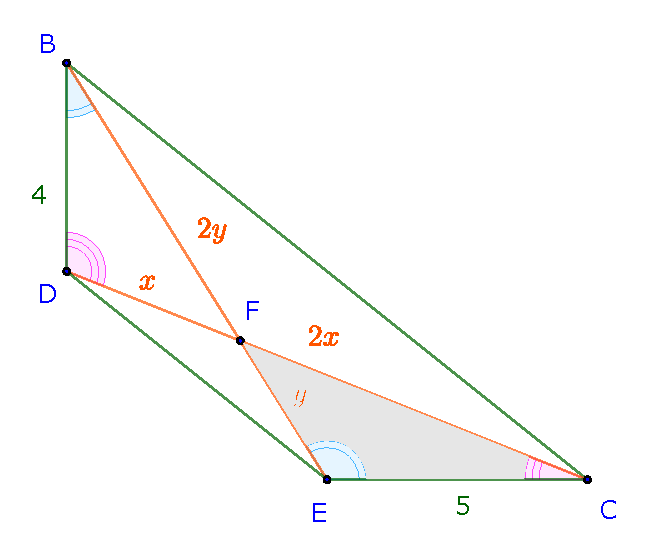
\includegraphics[width=6.5cm]{./svg/pdf/23-24-sm2-s4-ct-p3-2.pdf}
\end{center}

\bigbreak

\begin{problem}[Problem Four]
    Find one pair of positive integers $x, y$  such that $x^2 + 3y$ are $y^2 + 3x$ are perfect squares.

    Find all pairs of integers $(x, y)$ such that $x^2 + 3y$ and $y^2 + 3x$ are perfect squares.
\end{problem}

\bigbreak

\begin{problem}[Problem Five]
    $a, b$ are arbitrary positive real numbers. $x, y$ are real numbers such that 
    \[
        ax^2 + by^2 = ab.
    \]

    What is the value of $x+y$ when $xy$ reaches maximal value?
\end{problem}

\bigbreak

\begin{problem}[Problem Six]
    Find the minimal value of the following expression
    \[
        |x - 1| + |x - 2|.
    \]

    Find the minimal value of the following expression
    \[
        |x - 1| + |x - 2| + |x - 4| + \ldots + |x - 2^{2024}|.
    \]
\end{problem}

\bigbreak

\begin{problem}[Problem Seven]
    $ABCD$ is a rectangle where $AB=a,$ $AD=b,$ and $b>a.$ $P$ and $Q$ are points on $BD$ and $BC,$ respectively.
    Find the minimal value of $CP + PQ.$
\end{problem}

\begin{center}
    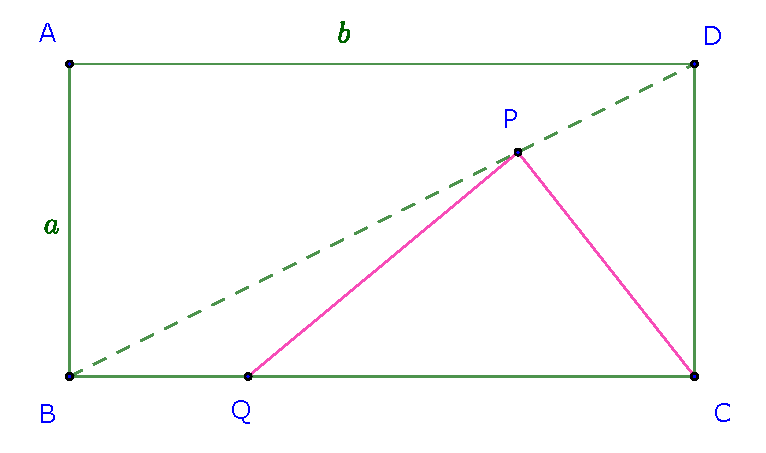
\includegraphics[width=6.5cm]{./svg/pdf/23-24-sm2-s4-ct-p3-7.pdf}
\end{center}

\bigbreak

\begin{problem}[Problem Eight]
    Find the maximal value of $2\sin^4{x}\cos^2{x}.$

    Find the maximal value of $\cos^3{x} + \sin^2{x} - \cos{x}.$
\end{problem}

\bigbreak

\begin{problem}[Problem Nine]
    $A, B, P$ are points on the perimeter of the unit circle centred at $O$ such that $\angle APB = \angle AOB.$
    Find the length of the chord $AB.$
\end{problem}

\begin{center}
    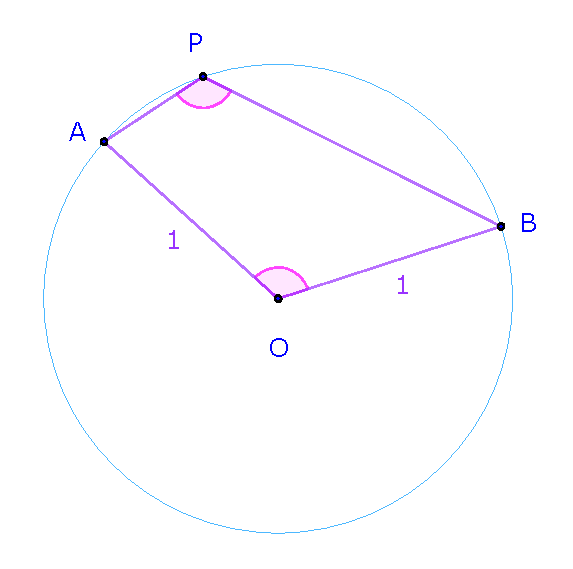
\includegraphics[width=6.5cm]{./svg/pdf/23-24-sm2-s4-ct-p3-9.pdf}
\end{center}

\bigbreak

\begin{problem}[Problem Ten]
    The sequence $(a_n)$ is defined as follow:
    \[
        a_0 = 2,\ a_{n+1} = 5a_n + \sqrt{24a_n^2 - 96},\ \forall n \ge 0.
    \]
    
    Find $a_{2024}.$
\end{problem}

\newpage

\section{Solutions}

\begin{problem}[Problem One]
    Find the value of:
    \[
        \left(4 + 2\sqrt{3}\right)^{\frac{3}{2}} - \left(4 - 2\sqrt{3}\right)^{\frac{3}{2}}
    \]
\end{problem}

\begin{soln}
    Note that 
    \[
        \begin{aligned}
            &4+2\sqrt{3} = (\sqrt{3})^2 - 2(\sqrt{3})(1) + 1^2 = (\sqrt{3}+1)^2,\ 4-2\sqrt{3} = (\sqrt{3}-1)^2\\
            &\Rightarrow \left(4 + 2\sqrt{3}\right)^{\frac{3}{2}} = (\sqrt{3}+1)^3,\ \left(4 - 2\sqrt{3}\right)^{\frac{3}{2}} = (\sqrt{3}-1)^3
        \end{aligned}
    \]

    Now, it is easy to see that for any real number $a:$
    \[
        \begin{aligned}
            &(a+1)^3 - (a-1)^3 = (a^3 + 3a^2 + 3a + 1) - (a^3 - 3a^2 + 3a - 1) = 6a^2+2\\
            &\Rightarrow (\sqrt{3}+1)^3 - (\sqrt{3}-1)^3 = 6(\sqrt{3})^2 + 2 = \boxed{20.}
        \end{aligned}
    \]
\end{soln}

\begin{problem}[Problem Two]
    Minh, Ha-Anh, and Julie were having a snowball fight.
    Ha-Anh threw the first snowball. Then in response to every snowball that hit her, Minh threw six snowballs.
    Similarly, each time she was hit by a snowball, Julie threw five. Ha-Anh threw four each time she was hit.
    After a certain amount of time the game ended.
    If in total 13 snowballs missed their targets, how many snowballs each one of the players threw?

    (\textit{You can't throw a snowball at yourself and one snowball cannot hit two people.})
\end{problem}

\begin{soln}
    Let the amounts of snowballs that hit Minh, Ha-Anh, and Julie be $m, h,$ and $j,$ respectively,
    then $13 + m + h + j$ is the total amount of snowballs.
    Thus, the number of ball they throw is $6m + (4h + 1) + 5j,$ (note that Ha-Anh threw the first snowball).
    Therefore:
    \[
        13 + m + h + j = 6m + (4h + 1) + 5j \Rightarrow 5m + 3h + 4j = 12 \Rightarrow m \in \{0, 1, 2\}
    \]

    \textit{Case 1:} $m=0$ then $3h+4j=12,$ $h$ is even.
    If $h=0, j=3,$ only Ha-Anh was the only other player who threw some balls, and she threw a single snowball, it is impossible to hit Julie three times.
    If $h=4, j=0,$ then Ha-Anh was the only who threw some balls, she threw a fives snowballs, and hit herself four times. It's impossible.

    \textit{Case 2:} $m=1$ then $3h+4j=7.$ It is easy to see that $h=1, j=1.$ So how did it happen?
    The first snowball threw by Ha-Anh hit one of the other two girls (says A, B). That girl (A) one threw some balls:
    (i) one of them hit both Ha-Anh and another hit the remaining girl (B), triggering the responses from both girls that hit no one;
    (ii) one of them hit only Ha-Anh, Ha-Anh threw some snowballs that hit the remaining girl (B), triggering her response that hit no one;
    (ii) one of them hit only  the remaining girl (B), B threw some snowballs that hit Ha-Anh, triggering her response that hit no one.
    The game is ended in any case.

    It is easy to see that the numbers of snowballs were the same in every case: $\boxed{6, 5, 5}$
    (3 hits and 13 misses.)

    \textit{Case 3:} $m=2$ then $3h+4j=2.$ There is no solution for this case.
\end{soln}

\begin{problem}[Problem Three]
    $CBDE$ is a quadrilateral. $BD=4,$ $CE=5.$ $BE$ and $CD$ meet at $F$ such that $BF = 2FE$ and $CF = 2 FD.$ Furthermore
    \[
        \angle FEC - \angle FBD = \angle FDB - \angle FCE = 90\dg. 
    \]

    Find the area of $\triangle CEF.$
\end{problem}

\begin{soln}
    Extend $BD$ and $CE$ to meet at $A.$ $\angle BAC = \angle FEC - \angle FBD = \angle FDB - \angle FCE = 90\dg.$
    \begin{center}
        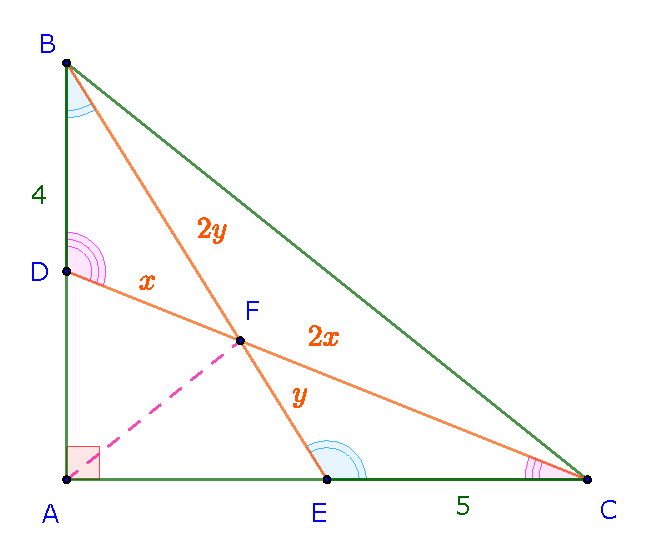
\includegraphics[width=6.5cm]{./svg/pdf/23-24-sm2-s4-ct-p3.pdf}
    \end{center}
    
    Let $s = [CEF], u = [AEF], v = [ADF],$ then
    \[
        \begin{aligned}
            &[BDF] = \half (FD)(FB) \sin{\angle DFB} = \half (x)(2y) \sin{\angle DFB} = \half (FC)(FE) \sin{\angle EFC} = s\\
            &[AEF] = \half [AFB] \Rightarrow u = \half(v + s),\ [ADF] = \half [AFC] \Rightarrow v = \half(u + s) \Rightarrow u=v=s\\
            &\Rightarrow D, E \text{\ are midpoints of\ } AB, AC \text{\ respectively} \Rightarrow DA = 8, AE = 10\\
            &[BCF] = 2 [FCE] = 2s \Rightarrow [ABC] = 6s \Rightarrow s = \frac{1}{6} [ABC] = \frac{40}{6} = \boxed{\frac{20}{3}.}
        \end{aligned}
    \]
\end{soln}

\begin{problem}[Problem Four]
    Find one pair of positive integers $x, y$  such that $x^2 + 3y$ are $y^2 + 3x$ are perfect squares.

    Find all pairs of integers $(x, y)$ such that $x^2 + 3y$ and $y^2 + 3x$ are perfect squares.
\end{problem}

\begin{soln}
    For the first question it is easy to see that $\boxed{x = y = 1}$ is a solution.

    Note that since $x, y$ are positive integers
    \[
        (x^2 + 3y) + (y^2 + 3x) < x^2 + 4x + 4 + y^2 + 4y + 4 = (x+2)^2 + (y+2)^2
    \]
    
    Thus one of the following is true: $x^2 + 3y < (x + 2)^2$ or $y^2 + 3x < (y+2)^2.$
    WLOG, $x^2 + 3y < (x + 2)^2,$ then since $x^2 + 3y > x^2,$ thus:
    \[
        \begin{aligned}
            &x^2 + 3y = (x+1)^2 \Rightarrow 3y = 2x+1 \Rightarrow y \text{\ is odd} \Rightarrow \exists k \ge 0:\ y = 2k+1 \Rightarrow x = 3k+1\\
            &y^2+3x = (2k+1)^2+3(3k+1) = 4k^2 + 13k + 4
            \Rightarrow
            \begin{cases}
                &4k^2 + 13k + 4 - (2k+3)^2 = k-5 > 0, \text{\ if\ } k\ge 6\\
                &4k^2 + 13k + 4 - (2k+4)^2 = -3k-12 < 0,\ \forall k\\
            \end{cases}
        \end{aligned}
    \]
    
    \textit{Case 1:} there are no solution if $k \ge 6.$

    \textit{Case 2:} if $k=5,$ then $x=16, y=11, x^2 + 3y = 289 = 17^2,$ $y^2+3x = 169=13^2.$

    \textit{Case 3:} $0< k < 5,$ it is easy to verify that there is no solution.

    \textit{Case 4:} $k = 0,$ $x^2 + 3y = 4 = 2^2,$ $y^2+3x = 4 = 2^2.$

    Thus, there are three solutions $\boxed{(1,1), (11, 16), (16, 11).}$
\end{soln}

\begin{problem}[Problem Five]
    $a, b$ are arbitrary positive real numbers. $x, y$ are real numbers such that 
    \[
        ax^2 + by^2 = ab.
    \]

    What is the value of $x+y$ when $xy$ reaches maximal value?
\end{problem}

\begin{soln}
    Note that
    \[
        \begin{aligned}
            &ax^2 + by^2 = ab \Rightarrow (\sqrt{a}x)^2 + (\sqrt{b}y)^2 - 2(\sqrt{a}x)(\sqrt{b}y) = ab - 2(\sqrt{a}x)(\sqrt{b}y)\\
            &\Rightarrow 2xy\sqrt{ab} = ab - (\sqrt{a}x - \sqrt{b}y)^2 \le ab.
        \end{aligned}
    \]

    $xy$ reaches the maximal value of $\frac{\sqrt{ab}}{2},$ when $\sqrt{a}x = \sqrt{b}y.$
    It is obvious that $x \ne 0, y \ne 0,$ so:
    \[
        y \frac{\sqrt{a}}{\sqrt{b}}x \Rightarrow ax^2 + b\left(\frac{\sqrt{a}}{\sqrt{b}}x\right)^2 = ab \Rightarrow 2ax^2 = ab \Rightarrow x = \pm \sqrt{\frac{b}{2}}, y = \pm \sqrt{\frac{a}{2}}
    \]

    Hence there are two values for $x+y:$ $\boxed{(\sqrt{\frac{b}{2}}, \sqrt{\frac{a}{2}}),\ (-\sqrt{\frac{b}{2}}, -\sqrt{\frac{a}{2}}).}$
\end{soln}

\begin{problem}[Problem Six]
    Find the minimal value of the following expression
    \[
        |x - 1| + |x - 2|.
    \]

    (\textit{8 points}) Find the minimal value of the following expression
    \[
        |x - 1| + |x - 2| + |x - 4| + \ldots + |x - 2^{2024}|.
    \]
\end{problem}

\begin{soln}
    It is easy to prove the following claim:
    \begin{claim*}
        $|x-a| + |x-b| \ge |a-b|, \text{\ the equality stands if\ } x \text{\ is between\ } a \text{\ and\ } b.$
    \end{claim*}

    For the first question,
    \[
        |x - 1| + |x - 2| \ge |1-2| = \boxed{1.}
    \]

    The equality stands when $x \in [1, 2].$

    Now,
    \[
        \begin{aligned}
            &|x - 2^i| + |x-2^{2024-i}| \ge |2^{2024-i} - 2^i| = 2^{2024-i} - 2^i,\ \forall i \in \{0, 1, \ldots, 1011\}\\
            &|x - 2^{2012}| \ge 0.
        \end{aligned}
    \]

    Thus, the minimal value of the expression is:
    \[
        \sum_{i=0}^{1011} (2^{2024-i} - 2^i) = (2^{1013}-1)(\sum_{i=0}^{1011} 2^i) = \boxed{(2^{1013}-1)(2^{2012}-1).}
    \]
    
    This, indeed, is reached when $x = 2^{2012}.$
\end{soln}

\newpage

\begin{problem}[Problem Seven]
    $ABCD$ is a rectangle where $AB=a,$ $AD=b,$ and $b>a.$ $P$ and $Q$ are points on $BD$ and $BC,$ respectively.
    Find the minimal value of $CP + PQ.$
\end{problem}

\begin{soln}
    Let $C'$ be the reflection of $C$ over $BD.$ Let $E$ be the foot of the perpendicular from $C'$ to $BC.$
    \begin{center}
        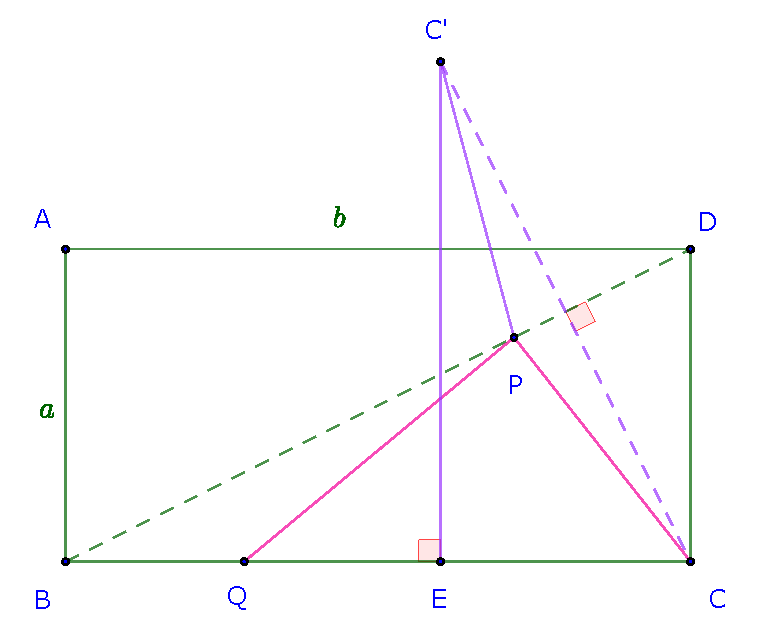
\includegraphics[width=6.5cm]{./svg/pdf/23-24-sm2-s4-ct-p3-7-2.pdf}
    \end{center}
    
    Then $CP + PQ = C'P + PQ \ge C'E.$
    \[
        \begin{aligned}
            &CC' \perp BD \Rightarrow C'C \cdot BD = 4[BCD] = 2\cdot BC \cdot CD \Rightarrow CC' = \frac{2ab}{\sqrt{a^2+b^2}}\\
            &\triangle CEC' \sim \triangle DCB \Rightarrow \frac{C'E}{CC'} = \frac{BC}{DB} \Rightarrow C'E = \frac{CC' \cdot BC}{BD} = \boxed{\frac{2ab^2}{a^2+b^2}.}
        \end{aligned}
    \] 
\end{soln}

\begin{problem}[Problem Eight]
    Find the maximal value of $2\sin^4{x}\cos^2{x}.$

    Find the maximal value of $\cos^3{x} + \sin^2{x} - \cos{x}.$
\end{problem}

\begin{soln}
    For the first question, by AM-GM:
    \[
        2\sin^4{x}\cos^2{x} = (\sin^2{x})(\sin^2{x})(2\cos^2{x}) \le \left( \frac{(\sin^2{x})+ (\sin^2{x}) + (2\cos^2{x}) }{3}\right)^3 = \boxed{\frac{8}{27}.}
    \]

    For the second question, let:
    \[
        \begin{aligned}
            &f(x) = \cos^3{x} + \sin^2{x} - \cos{x} = \sin^2{x} - \cos{x}(1-\cos^2{x}) = \sin^2{x}(1-\cos{x})\\
            &4 \sin^2{\frac{x}{2}}\cos^2{\frac{x}{2}} \cdot 2\sin^2{\frac{x}{2}} = 8 \sin^2{\frac{x}{2}}\sin^2{\frac{x}{2}}\cos^2{\frac{x}{2}}
        \end{aligned}
    \]

    By result of the first part, $f(x) \le 4 \frac{8}{27} = \boxed{\frac{32}{27}.}$
\end{soln}

\newpage

\begin{problem}[Problem Nine]
    $A, B, P$ are points on the perimeter of the unit circle centred at $O$ such that $\angle APB = \angle AOB.$
    Find the length of the chord $AB.$
\end{problem}

\begin{soln}
    Let $C$ be point on the major arc $AB.$ 
    \begin{center}
        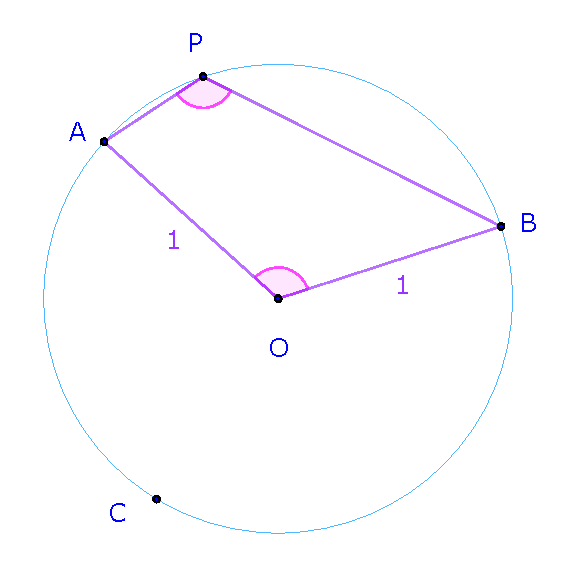
\includegraphics[width=6.5cm]{./svg/pdf/23-24-sm2-s4-ct-p3-9-2.pdf}
    \end{center}
    
    It is easy to see that:
    \[
        \arc{APB} = \angle {AOB} = \angle {APB} = \half \arc{ACB} = \half(360\dg - \arc{APB})\Rightarrow \arc{APB} = 120\dg.
    \]

    By the Law of Cosines: $AB^2 = OA^2 + OB^2 - 2(OA)(OB) \cos{\angle AOB} = 3 \Rightarrow AB = \boxed{\sqrt{3}.}$
\end{soln}

\begin{problem}[Problem Ten]
    The sequence $(a_n)$ is defined as follow:
    \[
        a_0 = 2,\ a_{n+1} = 5a_n + \sqrt{24a_n^2 - 96},\ \forall n \ge 0.
    \]
    
    Find $a_{2024}.$
\end{problem}

\begin{soln}
    First, by isolating the square root and squaring both sides:
    \[
        a_{n+1} = 5a_n + \sqrt{24a_n^2 - 96} \Rightarrow (a_{n+1} - 5a_n)^2 = 24a_n^2 - 96 \Rightarrow a_{n+1}^2 - 10 a_n a_{n+1} + a_{n}^2 = -96 \quad (*)
    \]

    Similarly:
    \[
        a_{n+2}^2 - 10 a_{n+1} a_{n+2} + a_{n+1}^2 = -96 \quad (**)
    \]

    Now, it is easy to see that $a_0 = 2 > 0, a_{n+1} \ge 5a_n > a_n,$ thus $(a_n)$ is a strictly increasing sequence or $a_{n+2} > a_n.$
    Thus by (*) and (**), $a_{n+2}$ and $a_n$ are the two roots of:
    \[
        x^2 - 10 a_{n+1} a + a_{n+1}^2 + 96 = 0 \Rightarrow a_n + a_{n+2} = 10 a_{n+1} \Rightarrow a_{n+2} - 10a_{n+1} + a_n = 0, \forall n \ge 0.
    \]
    
    Thus the characteristic polynomial of the sequence $(a_n)$ is $x^2 - 10x+1=0,$ whose roots are $5 \pm 2\sqrt{6},$ thus the generic term can be expressed as:
    \[
        \begin{aligned}
            &a_n = c_1(5+2\sqrt{6})^n + c_2(5-2\sqrt{6})^n, \text{\ where } c_1, c_2 \text{\ are some constants.}\\
            &a_0 = 2, a_1 = 10 \Rightarrow c_1 = c_2 = 1 \Rightarrow a_n = (5+2\sqrt{6})^n + (5-2\sqrt{6})^n.
        \end{aligned}
    \]

    Therefore $a_{2024} = \boxed{(5+2\sqrt{6})^{2024} + (5-2\sqrt{6})^{2024}.}$
\end{soln}

\end{document}